%-------------------------------------------------------------------------------------------------------------------------------%
%*******************************************************************************************************************************%
%****************************************************** 'cs-examples.tex' ******************************************************%
%*******************************************************************************************************************************%
%-------------------------------------------------------------------------------------------------------------------------------%
\makeatletter                                   % Change @ -> catcode'@=11 (letter) for use in macro names/definition
%-------------------------------------------------------------------------------------------------------------------------------%
%*******************************************************************************************************************************%
%*************************************************** CS test Group commands ***************************************************%
%*******************************************************************************************************************************%
\gdef\pkgopts@TESTING%
{%
    \Chapter{Package Info}
    \PrintPackageList{}\\\par%
    \PrintChoicesInfo%\\
    %\PrintBoolOptionPairsInfo
    \@PKGTESTING@SUBHEADING{pkgopt queries/printing}%
    \PrintPkgOpts{fontname}
    \PrintPkgOpts{fontfamily}
    mylatex@valid@fontname@choiceval@options=\mylatex@valid@fontname@choicearray@options\\
    @doc@fontsize=\@doc@fontsize\\
    f@halfsize=\f@halfsize\\
    %mylatex@exampleDir=\mylatex@exampleDir\\
    mylatex@exampleDir=\pkgoptval{exampleDir}
}
%-------------------------------------------------------------------------------------------------------------------------------%
\gdef\ARGUMENTPARSINGS@TESTING%
{%
    \@PKGTESTING@HEADING{ARGUMENTPARSINGS@TESTING}%
    \@parse@split@csv@args@TESTING%
    \parsecsvgrouplist@TESTING%
    \csv@to@bsv@TESTING%
    \csvgrouplist@TESTING%
    \argpack@TESTING%
    \getcsvindex@TESTING%
    \@dup@item@csvlist@TESTING%
    \@modparse@TESTING%
    \misc@arg@parse@TESTING%
    %\@arg@forwarding@TESTING%
}
%-------------------------------------------------------------------------------------------------------------------------------%
\gdef\XSV@LISTS@TESTING%
{%
    \@PKGTESTING@HEADING{XSV@LISTS@TESTING}%
    \@PKGTESTING@SUBHEADING{XSV list creation}%
    \@def@label@colors
    \createxsvargs{csv}{\@managed@counters}%
    %\meaning\@xsvargs@numformat%\xsvarg@numeral
    \csvargi%
    \csdefnumname@TESTING%
    \@PKGTESTING@SUBHEADING{XSV list usage}%
    \csvdirpath*{ion,{pCT\_code},git,\vardir*{GitHub account},\vardir*{GitHub repository}}\\%, $\dots$
    \csvdirpath{ion,{pCT\_code},git,\vardir*{GitHub account},\vardir*{GitHub repository}}+%, $\dots$
    \dirpath
}
%-------------------------------------------------------------------------------------------------------------------------------%
\gdef\CONDITIONALS@TESTING%
{%
    \@PKGTESTING@HEADING{CONDITIONALS@TESTING}%
    \cssetTF@TESTING%
    \csregsetTF@TESTING%
    \TFcompare@TESTING%
    \ifTFdo@TESTING%
    \if@X@TESTING
    \negated@if@X@TESTING%
    \IfXEqCase@TESTING%
    \do@once@TESTING%
}
%-------------------------------------------------------------------------------------------------------------------------------%
\gdef\REGVAR@TESTING%
{%
    \@PKGTESTING@HEADING{REGVAR@TESTING}%
    \theX@regprint@TESTING
    \@set@varname@reg@TESTING
    \@zsavepos@TESTING
    \@space@TESTING
    \@measure@text@TESTING%
    \@init@X@TESTING%          %def
    \@setcountval@X@TESTING%
}
%-------------------------------------------------------------------------------------------------------------------------------%
\gdef\TEXTPAR@TESTING%
{%
    \@PKGTESTING@HEADING{TEXTPAR@TESTING}%
    \numToText@TESTING%
    %\printnumber{\roman}{41}\\
    \ul@TESTING
}
%-------------------------------------------------------------------------------------------------------------------------------%
\gdef\MATH@TESTING%
{%
    \@PKGTESTING@HEADING{MATH@TESTING}%
    \def\setme{\afterassignment\setmeA\count255}
    \def\setmeA{$\number\count255\advance\count255 by 10
    +10=\number\count255$}
    Some arithmetic: \setme = 27
    \def\myarray{7,-3,4,-9,11}
    \pgfmathparse{{\myarray}[3]} \pgfmathresult
    \def\myarray{{"a","b","c","d","e"}}
    \pgfmathparse{\myarray[3]} \pgfmathresult
}
%-------------------------------------------------------------------------------------------------------------------------------%
\gdef\COLOR@TESTING%
{%
    \@PKGTESTING@HEADING{COLOR@TESTING}%
    \@color@shade[coltest]{green}
    \@color@shade[coltest]{green}+
    \@color@shade[coltest]{green}-
    \@color@shade[coltest]{green}+-
    \@PKGTESTING@SUBSUBHEADING{Custom color mix/set definitions}%
    @defined@colormixes=\@defined@colormixes\\%
    @defined@colorsets=\@defined@colorsets\\%
    @defined@tcbcolorsets=\@defined@tcbcolorsets\\%
}
%-------------------------------------------------------------------------------------------------------------------------------%
\gdef\TEMP@MISC@TESTING%
{%
    \@PKGTESTING@HEADING{Misc. Temporary Testing}%
    \foreach \@split@csv@args@cmd@type [count=\@csv@arg@index from 1] in {1..6}%
    {%
            \Romannumeral{\@csv@arg@index}
    }
}
%-------------------------------------------------------------------------------------------------------------------------------%
%*******************************************************************************************************************************%
%************************************ Control sequence and package testing content/commands ************************************%
%*******************************************************************************************************************************%
%-------------------------------------------------------------------------------------------------------------------------------%
%-------------------------------------------------------------------------------------------------------------------------------%
%-------------------------------------------------------------------------------------------------------------------------------%
%-------------------------------------------------------------------------------------------------------------------------------%
%\ARGUMENTPARSINGS@TESTING
%-------------------------------------------------------------------------------------------------------------------------------%
\gdef\@parse@split@csv@args@TESTING%
{%
        \@PKGTESTING@SUBHEADING{split csv arg parsing}%
        \gdef\defmid{defmid}%
        \gdef\argin{argin}%
        \gdef\argmid{argmid}%
        \gdef\argout{argout}%
        \setlength\@saved@length{1.5pt}%
        \setlength\@macro@height{2.5pt}%
        \setlength\@macro@length{2.5pt}%
        %-----------------------------------------------------------------------------------------------------------------------%
        \@parse@split@csv@args{setlength}<\@saved@length,\@macro@height,\@saved@length>=<\@macro@height,\@saved@length,\@macro@height>%
        1=$>$\the\@saved@length\\%
        2=$>$\the\@macro@height\\%
        %-----------------------------------------------------------------------------------------------------------------------%
        \@parse@split@csv@args{let}<argmid,argin,argout>=<argin,argout,argmid>%
        argin=$>$\argin\\%
        argmid=$>$\argmid\\%
        argout=$>$\argout\\%
        \@parse@split@csv@args{gdef}<defmid>=<\arabic{@macro@counter}>%
        %\@parse@split@csv@args{gdef}<defmid>=<12>%
        \@parse@split@csv@args{gdef}<csdefmid>=<\arabic{@macro@counter}>%
        defmid=$>$\defmid\\%
        %-----------------------------------------------------------------------------------------------------------------------%
        \setcounter{@macro@counter}{4}%
        \def\cmdlist{let,def,setlength}%
        \def\leftsplitarglist{<argout,defmid,\@saved@length>}%
        \def\rightsplitarglist{<argmid,\roman{@macro@counter},14pt>}%
        %\xp\xp\xp\def\xp\xp\xp\splitarglist\xp\xp\xp{\xp\xp\leftsplitarglist\rightsplitarglist}
        %\def\splitarglist{<argout,defmid,\@saved@length>=<argmid,\roman{@macro@counter},14pt>}
        \xp\xp\xp\xp\xp\xp\xp\@parse@split@csv@args\xp\xp\xp\xp\xp\xp\xp{\xp\xp\xp\cmdlist\xp\xp\xp}\xp\leftsplitarglist\xp=\rightsplitarglist%
        %\xp\xp\xp\@parse@split@csv@args\xp\xp\xp{\xp\cmdlist\xp}\splitarglist%
        %\xp\@parse@split@csv@args\xp{\cmdlist}<argout,defmid,\@saved@length>=<argmid,\roman{@macro@counter},14pt>%
        argout=$>$\argout\\%
        defmid=$>$\defmid\\%
        @saved@length=$>$\the\@saved@length%
}
%-------------------------------------------------------------------------------------------------------------------------------%
\gdef\parsecsvgrouplist@TESTING%
{%
    \@PKGTESTING@SUBHEADING{Parsecsvgroups}%
    \@PKGTESTING@SUBSUBHEADING{Comma-Separated Parentheses/Bracket/Brace Groups}%
    \@PKGTESTING@SUBHEADING{parsecsvgroups}%
    \parsecsvgrouplist(3,0,10),(3,1),(2,1),(2,2),(2,3),(1,3),(1,4);%
    \parsecsvgrouplist{3,0},{3,1},{2,1,14},{2,2},{2,3},{1,3},{1,4},{1,5};%
    \parsecsvgrouplist[3,0],[3,1],[2,1,13],[2,2],[2,3],[1,3],[1,4];%
    \@PKGTESTING@SUBHEADING{parsecsvgroups}%%
    \@PKGTESTING@SUBSUBHEADING{Mixed Parse Group}%
    \@PKGTESTING@SUBHEADING{parsecsvgroups}%
    \parsecsvgrouplist'\printcsvgroup'{3,0},[3,1],[2,1,14],(2,2),{2,3,12},(1,3,912),[1,4],{1,5};%
    \parsecsvgrouplist'\parsecsvgroup'{3,0},[3,1],[2,1,14],(2,2),{2,3,12},(1,3,912),[1,4],{1,5};%
}
%-------------------------------------------------------------------------------------------------------------------------------%
\gdef\csv@to@bsv@TESTING%
{%
    \@PKGTESTING@SUBHEADING{xsv group conversions}%
    \@PKGTESTING@SUBSUBHEADING{comma$\to$braces}%
    %\csv@to@bsv+
    \csv@to@bsv*<E,F,G,H>
    \def\csv@to@bsv@args{E,F,G,H}%
    \csv@to@bsv*<\csv@to@bsv@args>
    \csv@to@bsv*+<E,F,G,H>
}
%-------------------------------------------------------------------------------------------------------------------------------%
\gdef\csvgrouplist@TESTING%
{%
    \@PKGTESTING@SUBHEADING{csvlist: unique add/del}%
    \@uniquely@add@to@csvlist{test}{\uniquecsvtest}%
    \@uniquely@add@to@csvlist{testA}{\uniquecsvtest}%
    \@uniquely@add@to@csvlist{test}{\uniquecsvtest}%
    \@uniquely@add@to@csvlist{testB}{\uniquecsvtest}%
    \@uniquely@add@to@csvlist{test}{\uniquecsvtest}%
    \uniquecsvtest
    \@PKGTESTING@SUBHEADING{csv(e,g,x)del}%
    \csvxdel{\uniquecsvtest}{helo}%
    \uniquecsvtest
    \@PKGTESTING@SUBHEADING{create/add to/appending csvgrouplists}%
    \gdef\appendingcsvgroupA{num1,num2,num3,num4}%,\Large
    \gdef\appendingcsvgroupB{numa,numb,numc,numd}%,\Large
    \gdef\appendingcsvgroupC{numA,numB,numC,numD}%,\Large
    %
    \@PKGTESTING@SUBSUBHEADING{create@csvgroup}%
    %\def\thecsvgroupinitializer{num1,num2,num3,num4,\Large\def\plz{num5},num6}%,\Large
    %\create@csvgrouplist{\appendingcsvgroupA}%{num1,num2,num3,num4}%,num5,num6
    \create@csvgrouplist{\appendingcsvgroupA}%{num1,num2,num3,num4}%,num5,num6
    %newcsvgrouplist=\newcsvgrouplist\\%plz\\
    thecsvgroup=\thecsvgroup\\%plz\\(newcsvgrouplist)
    \create@csvgrouplist(csnamecsvgroup){\appendingcsvgroupA}%{num1,num2,num3,num4}%,num5,num6
    %newcsvgrouplist=\newcsvgrouplist\\%plz\\
    csnamecsvgroup=\csnamecsvgroup%plz\\(newcsvgrouplist)
    \@PKGTESTING@SUBSUBHEADING{add@to@csvgrouplist (create if undef)}%
    %\def\thecsvgrouptest{(num1)}%
    \add@to@csvgrouplist{\thecsvgrouptest}{num1}%
    \add@to@csvgrouplist{\thecsvgrouptest}{num2}%
    \add@to@csvgrouplist{\thecsvgrouptest}{num3}%
    \add@to@csvgrouplist{\thecsvgrouptest}{num4}%
    thecsvgrouptest=\thecsvgrouptest%
    %\xp\parsecsvgrouplist\thecsvgrouptest;
    \@PKGTESTING@SUBSUBHEADING{csvgrouplist@distribute@csv (create if undef)}%
    \csvgrouplist@distribute@csv{\thecsvgroup}{\appendingcsvgroupB}%
    %\create@csvgrouplist{\appendingcsvgroupA}%{num1,num2,num3,num4}%,num5,num6
    thecsvgroup=\thecsvgroup\\%plz\\
    %\printcsvgrouplist
    \csvgrouplist@distribute@csv{\thecsvgroup}{\appendingcsvgroupC}%
    thecsvgroup=\thecsvgroup%
    \@PKGTESTING@SUBSUBHEADING{csv@groups@to@grouplist}%
    \csvlists@to@grouplist{\appendingcsvgroupA,\appendingcsvgroupB,\appendingcsvgroupC}%
    thecsvgroup=\csvgroupslist
}
%-------------------------------------------------------------------------------------------------------------------------------%
%->
\def\lastvargcmdtest#1#2#3%
{%
        \@PKGTESTING@SUBSUBHEADING{lastvargcmd (argpack u\{-\} arg)}%
        \def\@print@arg@by@num@one{#1}%
        \def\@print@arg@by@num@two{#2}%
        \def\@print@arg@by@num@three{#3}%
        1=\@print@arg@by@num@one\\%
        2=\@print@arg@by@num@two\\%
        3=\@print@arg@by@num@three%
}
%-------------------------------------------------------------------------------------------------------------------------------%
\gdef\argpack@TESTING%
{%
    \@PKGTESTING@SUBHEADING{ARGPACK TESTING}%
    \argpack%
        {\@csv@grouped@arg@testlist}%
        \lastvargcmdtest{one}{two}{\romanarg{1}}-%
        {%
            argi=\romanarg{1}\\%
            argii=\romanarg{2}\\%
            argiii=\romanarg{3}\\%
            lastvarg=\lastvargcmd%
        }%
}
%-------------------------------------------------------------------------------------------------------------------------------%
\gdef\getcsvindex@TESTING%
{%
    \@PKGTESTING@SUBHEADING{getCSVindex}%
    \getcsvindex*{5}{\@csv@arg@testlist}\\
    \getcsvindex*={13}{{a,b,c,d,e,f,g,h,i,j,k}}\\
    \getcsvindex*=@{9}{\@csv@arg@testlist}\\
    \getcsvindex{12}{\@csv@arg@testlist}\\
    \getcsvindex*{12}{\@csv@arg@testlist}\\
    \getcsvindex*=@{14}{\@csv@arg@testlist}
}%
%-------------------------------------------------------------------------------------------------------------------------------%
\gdef\@dup@item@csvlist@TESTING%
{%
    \@PKGTESTING@SUBHEADING{@dup@item@csvlist}%
    \setcsvargs{\@csv@arg@testlist}%
    \@dup@item@csvlist*{\@csv@arg@testlist}{\@csv@arg@partial@testlist}{\@csv@arg@filled@testlist}%
    \@dup@item@csvlist*={\narg}{\@csv@arg@partial@testlist}{\@csv@arg@filled@testlist}%
    \@dup@item@csvlist*={\narg}{A}%
    \@dup@item@csvlist*{\@csv@arg@testlist}{A}%
    \@dup@item@csvlist*{\@csv@arg@testlist}{A}{\@csv@arg@filled@testlist}%
}%
%-------------------------------------------------------------------------------------------------------------------------------%
\gdef\@modparse@TESTING%
{%
    \@PKGTESTING@SUBHEADING{mod parse brace separated value argument lists}%
    \@modparse@bsv@args{2}{{A}{B}{C}{D}{E}{F}{G}{H}}{argi=\bsvargi,argii=\bsvargii\\}
    \@modparse@bsv@args{2}{\@braced@arg@testlist}{argi=\bsvargi,argii=\bsvargii}
}
%-------------------------------------------------------------------------------------------------------------------------------%
\gdef\misc@arg@parse@TESTING%
{%
    \@PKGTESTING@SUBHEADING{misc arg parsing}%
    \makecsv*{a,b,c,d,e,f,g}
    \printcsv{\l@myvararg@parameters@clist}
    \printargs{csv}{\@csv@arg@testlist}
    \printargs{bsv}{{A}{B}{C}{D}{E}{F}{G}{H}}
    \printargs{ssv}{\@spaced@arg@testlist}
    \@csvlist@length*[@TF@indicator@typesB]{\@TF@indicator@types}\\
    \@TF@indicator@typesB@length
}
%-------------------------------------------------------------------------------------------------------------------------------%
\gdef\@arg@forwarding@TESTING%
{%
    \@PKGTESTING@SUBHEADING{Forwarding Arguments to Submacros}%
    \DeclareDocumentCommand{\cprinttest}{s t! m}
    {%{manual print on}{print statement}
            \IfBooleanTF{##1}{RegT}{RegF}%
            %\IfSubBooleanTF{#1}{SubT}{SubF}%
            \IfBooleanTF{##2}{xRegT}{xRegF}%
            %\IfSubBooleanTF{#2}{xSubT}{xSubF}%
            3=##3\\
    }
    \forwardBooleanMixList{\cprinttest}{\BooleanTrue/*/TF,\BooleanTrue/!/FT}{T}{F}\\
    \forwardBooleanMixList{\cprinttest}{\BooleanTrue/*/TF,\BooleanFalse/!/FT}{T}{F}\\
    \forwardBooleanMixList{\cprinttest}{\BooleanFalse/*/TF,\BooleanTrue/!/FT}{T}{F}\\
    \forwardBooleanMixList{\cprinttest}{\BooleanFalse/*/TF,\BooleanFalse/!/FT}{T}{F}
}
%-------------------------------------------------------------------------------------------------------------------------------%
%-------------------------------------------------------------------------------------------------------------------------------%
%-------------------------------------------------------------------------------------------------------------------------------%
%-------------------------------------------------------------------------------------------------------------------------------%
%\XSV@LISTS@TESTING
%-------------------------------------------------------------------------------------------------------------------------------%
\gdef\csdefnumname@TESTING%
{%
    \@PKGTESTING@SUBHEADING{csdefnumname/thecsnumname TESTING}%
    \varul{\textbf{Description:}} csdefnumname/thecsnumname commands have modifiable prefix (default:'arg'), may include an optional suffix, and Boolean arg specification of name/ordinal/fraction text numname\\
    %\@PKGTESTING@SUBHEADING{default def/print}%
    \csdefnumname{1}{argone def text}%
    \csdefnumname{2}{argtwo def text}%
    csnumname1=\thecsnumname{1}\\%
    csnumname2=\thecsnumname{2}%
    \@PKGTESTING@SUBSUBHEADING{numname=num@to@ordinal}%
    \emph{define:}\\
    %\setprint{\BooleanTrue}%
    arg2(!)=\csdefnumname(!){2}{hello 1}\\%
    arg2here(*)=\csdefnumname*{2}/here/{hello 2}\\%
    arg3=\csdefnumname{3}{hello 1}\\%
    arg3here=\csdefnumname{3}/here/{hello 2}\\%
    arg4=\csdefnumname{4}{hello 1}\\%
    arg4here=\csdefnumname{4}/here/{hello 2}\\%
    \emph{use:}\\
    argtwo=\csuse{argtwo}\\
    argtwohere=\csuse{argtwohere}\\
    argthree=\csuse{argthree}\\%
    argthreehere=\csuse{argthreehere}\\%
    argfour=\csuse{argfour}\\
    argfourhere=\csuse{argfourhere}
    \@PKGTESTING@SUBSUBHEADING{numname=num@to@ordinal}%
    \emph{define:}\\
    thearg2(+)=\csdefnumname(+){2}|thearg|{hello 1}\\%
    thearg2here(+)=\csdefnumname(+){2}|thearg|/here/{hello 2}\\%
    thearg4(!+)=\csdefnumname(!+){4}|thearg|{hello 1}\\%
    thearg4here(+)=\csdefnumname(+){4}|thearg|/here/{hello 2}\\%
    \emph{use:}\\
    theargsecond=\csuse{theargsecond}\\
    theargsecondhere=\csuse{theargsecondhere}\\
    theargfourth=\csuse{theargfourth}\\
    theargfourthhere=\csuse{theargfourthhere}
    \@PKGTESTING@SUBSUBHEADING{num@to@fraction}%
    \emph{define:}\\
    thearg12=\csdefnumname{1}'2'|thearg|{hello 12}\\%
    thearg32(+)=\csdefnumname(+){3}'2'|thearg|{hello 32}\\%
    thearg12here=\csdefnumname{1}'2'|thearg|/here/{hello 12}\\%
    thearg14(!)=\csdefnumname(!){1}'4'|thearg|{hello 14}\\%
    thearg14here=\csdefnumname{1}'4'|thearg|/here/{hello 14}\\%
    thearg14here(+)=\csdefnumname(+){1}'4'|thearg|/here/{hello 14}\\%
    thearg34here=\csdefnumname{3}'4'|thearg|/here/{hello 34}\\%
    \emph{use:}\\
    theargonehalf=\csuse{theargonehalf}\\
    theargthreehalves=\csuse{theargthreehalves}\\
    theargonehalfhere=\csuse{theargonehalfhere}\\
    theargonequarter=\csuse{theargonequarter}\\
    theargonequarterhere=\csuse{theargonequarterhere}\\
    theargthreequartershere=\csuse{theargthreequartershere}
    \@PKGTESTING@SUBSUBHEADING{xsvargdef/thexsvarg}%
    \csvargdef{1}{csvargdef test}%
    \csvargi\\%
    \thexsvarg{csv}{1}\\%
    %\setcsvargs[\roman]\@csv@arg@partial@testlist
    thenumname=\thenumname{@macro@counter}\\
    %thenumname=\thenumnamenumeral{@macro@counter}
    %\csvargdef[\thenumname]{1}{csvargdef test}%
    %\csvargi\\%
}
%-------------------------------------------------------------------------------------------------------------------------------%
%-------------------------------------------------------------------------------------------------------------------------------%
%-------------------------------------------------------------------------------------------------------------------------------%
%-------------------------------------------------------------------------------------------------------------------------------%
%\CONDITIONALS@TESTING
%-------------------------------------------------------------------------------------------------------------------------------%
\gdef\cssetTF@TESTING%
{%
    %\@equality@status@true
    \@PKGTESTING@SUBHEADING{cssetTF}%
    \@PKGTESTING@SUBSUBHEADING{@equality@status@true/false (w/o explicit TF value)}%
    TFtest(F) =\cssetTF*{TF}{TFtest}\\
    @macro@if(F) =\cssetTF*{2}{@macro@if}\\
    @macro@toggle(F) =\cssetTF*{3}{@macro@toggle}\\
    binarytest(F) =\cssetTF*{4}{binarytest}\\
    @macro@counter(F) =\cssetTF*{5}{@macro@counter}
    %--------------------------------------------------------------------------------------------------------------------------%
    \@PKGTESTING@SUBSUBHEADING{EXPLICIT SET}%
    @macro@toggle(T) =\thetoggleval{@macro@toggle}\\
    @macro@if(T) =\ifval{@macro@if}\\
    \toggletrue{@macro@toggle}
    \booltrue{@macro@if}
    TFtest(T) =\cssetTF*[@macro@toggle]{TF}{TFtest}\\
    TrueFalsetest(T) =\cssetTF*[@macro@if]{TrueFalse}{TrueFalsetest}\\
    @macro@if(T) =\cssetTF*[@boolean@true@counter]{if}{@macro@if}\\
    @macro@toggle(F) =\cssetTF*[\BooleanFalse]{toggle}{@macro@toggle}
    %--------------------------------------------------------------------------------------------------------------------------%
    \@PKGTESTING@SUBSUBHEADING{DEFAULT SET}%
    @macro@counter(F) =\cssetTF*{5}{eq@ifstrequallist}\\
    xparsetest(F) =\cssetTF*{6}{eq@ifstrequallist}
    %--------------------------------------------------------------------------------------------------------------------------%
    \@PKGTESTING@SUBSUBHEADING{@print@conditional}%
    @macro@toggle=\@print@conditional{@macro@toggle}{TF}\\
    @macro@toggle=\@print@conditional!{@macro@toggle}{xparse}\\
    @macro@if=\@print@conditional{@macro@if}{binary}\\
    @macro@counter=\@print@conditional{@macro@counter}{if}\\
    TFtest=\@print@conditional{TFtest}{TF}%
}
%-------------------------------------------------------------------------------------------------------------------------------%
\gdef\csregsetTF@TESTING%
{%
    \@PKGTESTING@SUBHEADING{csregsetTF TESTING}%
    \csregsetTF*{@macro@toggle}{0} (F)\\
    \csregsetTF*{@macro@toggle}{\BooleanTrue} (T)\\
    \csregsetTF*{@macro@toggle}{false} (F)\\
    \csregsetTF*{@macro@toggle}{@boolean@true@toggle} (T)
}
%-------------------------------------------------------------------------------------------------------------------------------%
\gdef\TFcompare@TESTING%
{%
    \conditional{\ifnumcomp{\value{@macro@counter}}{=}{2}}{numcomp}{no numcomp}\\
    \conditional{\ifdefined\asasasf@size}{defined}{not defined}
    %\conditional{\ifmylatex@FBM@clearpage}{ifmylatex@FBM@clearpage}{not ifmylatex@FBM@clearpage}\\
    \@PKGTESTING@SUBHEADING{TFcomparisons}%
    TFcompare(F) =\TFcompare*{\binaryF}{\binaryT}\\%
    TFcompare(T) =\TFcompare*{\BooleanTrue}{\binaryT}\\%
    TFcompare(T) =\TFcompare{\@T@indicator}{\binaryT}\\%
    TFcompare(T) =\TFcompare*{\binaryF}{\@binary@F@indicator}%
}
%-------------------------------------------------------------------------------------------------------------------------------%
\gdef\ifTFdo@TESTING%
{%
    \@PKGTESTING@SUBHEADING{ifTFdo}%
    \ifTFdo{@macro@counter}{T}{F} (F)\\
    \ifTFdo{@macro@toggle}{T}{F} (F)\\
    \ifTFdo{@macro@if}{T}{F} (T)\\
    \ifTFdo{\BooleanTrue}{T}{F} (T)
}
%-------------------------------------------------------------------------------------------------------------------------------%
\gdef\if@X@TESTING%
{%
    \@PKGTESTING@SUBHEADING{if@X}%
    \@PKGTESTING@SUBSUBHEADING{Individual Conditionals}%
    ifismacro\{bshift\}=\ifismacro{\bshift}{macro}{not macro}\\
    ifismacro\{thebshift\}=\ifismacro{thebshift}{macro}{not macro}
    \@PKGTESTING@SUBSUBHEADING{Composite Conditionals}%
    \ifAnd%
    {%
        \ifdefined\pkgname/if,%         T
        \ifnumequal{1}{1}/TF,%        T
        \ifnumequal{0}{0}/TF,%        T
        \ifdefined\pkgopts/if,%         F
        \ifnumequal{1}{0}/TF%         F
    }%
    {ifAnd:=T}{ifAnd:=F} (F)\\%
    \ifXOr%
    {%
        \ifdefined\pkgname/if,%         T
        %\ifnumequal{1}{1}/TF,%       T
        %\ifnumequal{0}{0}/TF,%       T
        \ifdefined\pkgopts/if,%         F
        \ifnumequal{1}{0}/TF%         F
    }%
    {ifXOr:=T}{ifXOr:=F} (T)\\%
    \ifOr%
    {%
        \if@print@on@/if,%              F
        \if@local@print@on@/if%         F
    }%
    {ifOr:=T}{ifOr:=F}(F)%
}
%-------------------------------------------------------------------------------------------------------------------------------%
\gdef\negated@if@X@TESTING%
{%
    \@PKGTESTING@SUBHEADING{negated@if@X@TESTING}%
    \@PKGTESTING@SUBSUBHEADING{ifdefempty}%
    \def\emptydef{}%
    \def\nonemptydef{nonemptydef}%
    empty:\ifdefempty{\emptydef}{T}{F}\\
    empty(negated):\negate\ifdefempty{\emptydef}{T}{F}\\
    nonempty:\ifdefempty{\nonemptydef}{T}{F}\\
    nonempty(negated):\negate\ifdefempty{\nonemptydef}{T}{F}
    \@PKGTESTING@SUBSUBHEADING{ifdefunequal}%
    equal:\ifdefunequal{\emptydef}{\emptydef}{T}{F}\\
    equal(negated):\negate\ifdefequal{\emptydef}{\emptydef}{T}{F}\\
    unequal:\ifdefunequal{\nonemptydef}{\emptydef}{T}{F}\\
    unequal(negated):\negate\ifdefequal{\nonemptydef}{\emptydef}{T}{F}
}
%-------------------------------------------------------------------------------------------------------------------------------%
\gdef\IfXEqCase@TESTING%
{%
    \@PKGTESTING@SUBHEADING{If(X)EqCase}%
    \xdef\@IfCSEqCase@element{rparen}%
    \xdef\@IfDefEqCase@element{\rparen}%
    \@PKGTESTING@SUBSUBHEADING{IfCSEqCase}%
    \IfCSEqCase{\@IfCSEqCase@element}%
    {%
        {rparen}{\texttt{hello}\\\@namedef{thistest}{Hello $there$}\thistest}%
        {lparen}{D}%
        {dparen}{F}%
        {paren}{H}%
    }%
    \@PKGTESTING@SUBSUBHEADING{IfDefEqCase}%
    \IfDefEqCase{\@IfDefEqCase@element}%
    {%
        {\rparen}{\texttt{hello}\\\@namedef{thisDefEqCase}{Hello $there$}\thisDefEqCase}%
        {\lparen}{D}%
        {\thepage}{F}%
        {\vert}{H}%
    }%
}
%-------------------------------------------------------------------------------------------------------------------------------%
\gdef\do@once@TESTING%
{%
    \@PKGTESTING@SUBHEADING{do@once}%
    %\do@once{@measure@cfootpos}{herllo}\\
    %\do@once{@measure@cfootpos}{herllo}\\
    %\do@once{@measure@cfootpos}{herllo}\\
}
%-------------------------------------------------------------------------------------------------------------------------------%
%-------------------------------------------------------------------------------------------------------------------------------%
%-------------------------------------------------------------------------------------------------------------------------------%
%-------------------------------------------------------------------------------------------------------------------------------%
%\REGVAR@TESTING
%-------------------------------------------------------------------------------------------------------------------------------%
\gdef\theX@regprint@TESTING%
{%
    \@PKGTESTING@SUBHEADING{theX@regprint}%
    bigskipamount=\the\bigskipamount\\
    the@macro@length=\the@macro@length\\
    the@macro@toggle=\the@macro@toggle\\
    the@measure@cfootpos=\the@measure@cfootpos\\
    the@measure@pos=\the@measure@pos\\
    thebshift=\thebshift\\
    the@macro@skip=\the@macro@skip\\
    %-------------------------------------------------------------------------------------------------------------------------------%
    \booltrue{@macro@if}
    \toggletrue{@macro@toggle}
    \@print@bool@value{@macro@if}\\
    \@print@toggle@value{@macro@toggle}\\
    %-------------------------------------------------------------------------------------------------------------------------------%
    \begingroup%
    %\global\boolfalse{@macro@if}
    %\global\togglefalse{@macro@toggle}
    \g@boolfalse{@macro@if}%
    \g@togglefalse{@macro@toggle}%
    \@print@bool@value{@macro@if}\\
    \@print@toggle@value{@macro@toggle}\\
    \endgroup
    \@print@bool@value{@macro@if}\\
    \@print@toggle@value{@macro@toggle}
}
%-------------------------------------------------------------------------------------------------------------------------------%
\gdef\@set@varname@reg@TESTING%
{%
    \@PKGTESTING@SUBHEADING{@set@varname@reg}%
    \@set@varname@reg*{length}{testing}{@width}{26.35pt}\\%
    \@set@varname@reg*{length}{testvarlength}{@width}{5.0pt}\\
    \@set@varname@reg*{length}{mylatex@fontname}{@width}{5.0pt}\\
    \the\testvarlength@width\\
    \the\mylatex@fontname@width
}
%-------------------------------------------------------------------------------------------------------------------------------%
\gdef\@zsavepos@TESTING%
{%
    \@PKGTESTING@SUBHEADING{@zsavepos@TESTING}%
    \@print@zsavepos@pt{bottom@coverpage}\\
    \@print@zsavepos@pt{cfootpos}\\
    %ABC\\
    %\vfill\zsavepos{bottom@page}%
    %\printzsavepos{bottom@page}%
    %\clearpage
    \printzsavepos{bottom@page}\\%
    \printzsavepos{bottom@coverpage}\\%
    \printzsavepos{top@docpage}\\%
    \printzsavepos{cfootpos}%cfootpos
}
%-------------------------------------------------------------------------------------------------------------------------------%
\gdef\@space@TESTING%
{%
    \@PKGTESTING@SUBHEADING{fractional space dimension settings}%
    abc\tinyspace abc\tinyspace-abc\minispace abc\minispace-\\
    \setlength\@macro@length{\widthof{\tinyspace}}
    \the\@macro@length\\
    \setlength\@macro@length{\widthof{\minispace}}
    \the\@macro@length\\
    \setlength\@macro@length{\widthof{\space}}
    \the\@macro@length\\
    \the\space@length\\
    \the\fontdimen2\font plus \the\fontdimen3\font minus \the\fontdimen4\font\\
    \the\fontdimen2\font\space plus \the\fontdimen3\font\space minus \the\fontdimen4\font\\
    \the\fontdimen2\font\minispace plus \the\fontdimen3\font\minispace minus \the\fontdimen4\font\\
    \the\fontdimen2\font\tinyspace plus \the\fontdimen3\font\tinyspace minus \the\fontdimen4\font\\\\
    \def@fractional@spacing%\\
    onequarter@spacing=\onequarter@spacing\\
    onehalf@spacing=\onehalf@spacing\\
    threequarters@spacing=\threequarters@spacing\\
    threehalves@spacing=\threehalves@spacing\\
    onethird@spacing=\onethird@spacing\\
    twothirds@spacing=\twothirds@spacing\\
    fourthirds@spacing=\fourthirds@spacing\\
    sevenquarters@spacing=\sevenquarters@spacing
}
%-------------------------------------------------------------------------------------------------------------------------------%
\gdef\@measure@text@TESTING%
{%
    \@PKGTESTING@SUBHEADING{Text dimension measurements}%
    \@measure@text{x}[measure=letters,maxheight=true]%
        measure=letters,maxheight=true:@measure@text 2/3=\the\@premeasured@savebox@height\\
    \@measure@text{x}[measure=letters,maxheight=true,format=\LARGE, saveas=testsaveas]%
        measure=letters,maxheight=true,format=\LARGE, saveas=testsaveas:@measure@text testsaveas 2/3=\the\testsaveas@height\\
    \@measure@text[measure=letters,maxheight=true,format=\small,arg=x]%
        measure=letters,maxheight=true,format=\small,arg=x:@measure@text 2/3=\the\@premeasured@savebox@height\\
    \@measure@text[measure=numbers,maxheight=true,format=\tiny]%
        measure=letters,maxheight=true,format=tiny:@measure@text 2/3=\the\@premeasured@savebox@height\\
    \@measure@text[measure=letters,arg=X,format=\tiny]%
        measure=letters,arg=X,format=tiny:@measure@text 2/3=\the\@premeasured@savebox@height\\
    \@measure@text[measure=numbers,format=\LARGE]%
        measure=numbers,format=LARGE:@measure@text 2/3=\the\@premeasured@savebox@height\\
    %\@measure@text{\@axis@font@cmds x}%
    %    2:@measure@text 2=\the\@premeasured@savebox@height\\
    \@measure@text[measure=letters]%
        3:@measure@text 3=\the\@premeasured@savebox@height\\
    \@measure@text%
        none:@measure@text none=\the\@premeasured@savebox@height
}
%-------------------------------------------------------------------------------------------------------------------------------%
\gdef\@init@X@TESTING%
{%
    \@PKGTESTING@SUBHEADING{@init@X}%
    %\@PKGTESTING@SUBSUBHEADING{@init@count}%
    \@init@count{\testcount}%
    \@PKGTESTING@SUBSUBHEADING{op(count)$\to$print(count)}%
    \printcount\testcount\\
    \stepcount\testcount%
    \printcount\testcount\\
    \addtocount\testcount{3}%
    \printcount\testcount\\
    \setcount\testcount{12}%
    \printcount\testcount\\
    \incrementcount\testcount%
    \printcount\testcount\\
    \decrementcount\testcount%
    \printcount\testcount
}
%-------------------------------------------------------------------------------------------------------------------------------%
\gdef\@setcountval@X@TESTING%
{%
    \@PKGTESTING@SUBHEADING{setcountval}%
    \setcountval*{\ONE}                 %def
    \setcountval*{ONE}                  %not def,ltxcounter,cscounter
    \setcountval*{@macro@counter}       %not def,ltxcounter,not cscounter
    \setcountval*{c@@macro@counter}     %not def,not ltxcounter,cscounter
    \setcountval*{\c@@macro@counter}    %def
    \setcountval*{3}          %-------------------------------------------------------------------------------------------------------------------------------%
}
%-------------------------------------------------------------------------------------------------------------------------------%
%-------------------------------------------------------------------------------------------------------------------------------%
%\TEXTPAR@TESTING
%-------------------------------------------------------------------------------------------------------------------------------%
\gdef\numToText@TESTING%
{%
    \@PKGTESTING@SUBHEADING{numToText}%
    \csgdef{testargone}{testargonedef}%
    \csgdef{onetestarg}{onetestarg}%
    \setcounter{@macro@counter}{1}%
    \@digits@to@name{\BooleanFalse}{@macro@counter}%
    \@the@digits@text\\%
    \csname testarg\@the@digits@text\endcsname%
    %\setprint!%
    \setprint!{\BooleanTrue}%
    %\setprint!{\BooleanFalse}%
    %\def\@xparse@T@indicator{\BooleanTrue}
    %\def\@xparse@F@indicator{\BooleanFalse}
    %---------------------------------------------------------------------------------------------------------------------------%
    \@PKGTESTING@SUBSUBHEADING{Ordinals}%
    \numToText+{0}\\
    \numToText!+*{0}\\
    \numToText+{4}\\
    \numToText+*{10}\\
    \numToText+*{14}\\
    \numToText+{40}\\
    \numToText+*{40}\\
    \numToText+{100}\\
    \numToText+{200}\\
    \numToText+{1000}\\
    \numToText+{124567}\\
    \numToText+{1234567}\\
    \numToText+{1000000000}\\
    \numToText+*{1000000000}\\
    \numToText+{1587134729}\\
    \numToText+*{1587134729}
    %---------------------------------------------------------------------------------------------------------------------------%
    \@PKGTESTING@SUBSUBHEADING{Fractions}%
    \numToFrac{1}{2}\\
    \numToText{1}{2}\\
    \numToText{1}{2}\\
    \numToText*{1}{2}\\
    %\numToFrac*{1}{2}\\
    \numToText{3}{2}\\
    \numToText*{3}{2}\\
    \numToText{3}{2}\\
    \numToText{3}{2}[sepfracs=true]\\
    \numToText{1}{3}\\
    \numToText{1}{4}\\
    \numToText*{1}{4}\\
    \numToText{3}{4}[sepfracs=true]\\
    \numToText*{1}{14}[sepfracs=true]\\
    \numToText{2}{104}\\
    \numToText!*{2}{104}\\
    \numToText!{2}{102}\\
    \numToText*{2}{102}\\
    \numToText{2}{120}\\
    \numToText*{2}{120}\\
    \numToText{2}{140}\\
    \numToText*{2}{140}\\
    \numToText{4}{40}\\
    \numToText*{4}{40}
    %---------------------------------------------------------------------------------------------------------------------------%
    \@PKGTESTING@SUBSUBHEADING{Names}%
    \numToText{0}[sepunits=true]\\
    \numToText!*{0}[sepunits=true]\\
    \numToText*{100}[sepitems=true, sepgroups=true, sepunits=true]\\
    \numToText*{1000}[sepitems=true, sepgroups=true, sepunits=true]\\
    \numToText*{10000}[sepitems=true, sepgroups=true, sepunits=true]\\
    \numToText*{100000}[sepitems=true, sepgroups=true, sepunits=true]\\
    \numToText*{1000000}[sepitems=true, sepgroups=true, sepunits=true]\\
    \numToText*{10000000}[sepitems=true, sepgroups=true, sepunits=true]\\
    \numToText{100729}[sepitems=true, sepgroups=true, sepunits=true]\\
    \numToText*{100729}[sepitems=true, sepgroups=true, sepunits=true]\\
    \numToText*{100729}\\
    \numToText{1000719}[sepitems=true, sepgroups=true, sepunits=true]\\
    \numToText*{1000719}[sepitems=true, sepgroups=true, sepunits=true]\\
    \numToText*{1000719}\\
    \numToText*{11127000}[sepgroups=true]\\
    \numToText{587000729}[sepgroups=true]\\
    \numToText{1000000000}[sepitems=true, sepgroups=true, sepunits=true]\\
    \numToText*{1000000000}[sepitems=true, sepgroups=true, sepunits=true]\\
    \numToText{1587134729}[sepitems=true, sepgroups=true, sepunits=true]\\
    \numToText*{1587134729}[sepitems=true, sepgroups=true, sepunits=true]
    %---------------------------------------------------------------------------------------------------------------------------%
    \@PKGTESTING@SUBSUBHEADING{Counter Ordinals}%
    \setcounter{@macro@counter}{0}%
    \numToText{@macro@counter}\\
    \setcounter{@macro@counter}{4}%
    \numToText{@macro@counter}\\
    \setxsvnumnames{csv}{@macro@counter}{\@managed@counters}%\\
    \csvargfouri\\
    %thenumname=\thenumname{@macro@counter}\\
    %thenumname=\thenumnamenumeral{@macro@counter}
}
\gdef\ul@TESTING%
{%
    \@PKGTESTING@SUBHEADING{ul@TESTING}%
    \varuline{varuline:Blupp of (that's \emph{of}, not \emph{off}, of course) a great Synopsis}\\
    \varul{varul:Blupp of (that's \emph{of}, not \emph{off}, of course) a great Synopsis}\\
    %\varuline{1.25pt}{.5pt}{1.25}{\sffamily Blupp of (that's \emph{of}, not \emph{off}, of course) a great Synopsis}\\
    \underline{underline:Blupp of (that's \emph{of}, not \emph{off}, of course) a great Synopsis}\\
    \tikzUL{tikzUL:Blupp of (that's \emph{of}, not \emph{off}, of course) a great Synopsis}\\
    \ul{ul:Blupp of (that's \emph{of}, not \emph{off}, of course) a great Synopsis}\\
    \uline{uline:Blupp of (that's \emph{of}, not \emph{off}, of course) a great Synopsis}
%\special{pdf:bcolor [.3 0 .3] [0.2]} % two arrays: first defines fill, second the stroke.
% If array has one entry, it's meaning grayscale, if three: RGB, if four: CMYK.
%\special{pdf:literal direct .1 w 2 Tr} % .4 here is the stroke width
%\pscharpath[fillstyle=solid,fillcolor=red]{hello}\\
%F
%\bye
}
%-------------------------------------------------------------------------------------------------------------------------------%
%*******************************************************************************************************************************%
%***************************************************** Group test commands *****************************************************%
%*******************************************************************************************************************************%
%-------------------------------------------------------------------------------------------------------------------------------%
%-------------------------------------------------------------------------------------------------------------------------------%
%*******************************************************************************************************************************%
%*******************************************************************************************************************************%
%*******************************************************************************************************************************%
%-------------------------------------------------------------------------------------------------------------------------------%
\def\@mbb@symbolsTest%
{%
    $\bbGamma\bbDelta\bbTheta\bbLambda\bbXi\bbPi\bbSigma\bbUpsilon\bbPhi\bbPsi\bbOmega\bbalpha\bbbeta\bbgamma\bbdelta\bbespilon%
    \bbzeta\bbeta\bbtheta\bbiota\bbkappa\bblambda\bbmu\bbnu\bbxi\bbpi\bbrho\bbsigma\bbtau\bbupsilon\bbphi\bbchi\bbpsi\bbomega$%
    %%$\Bbbsumop\Bbbsum$\\
}
%-------------------------------------------------------------------------------------------------------------------------------%
\def\@symbols@Test%
{%
    \victorysym\\
    %%$\phiup$\male\female\currency\phone\recorder\clock\lightning\pointer\RIGHTarrow\LEFTarrow\UParrow\DOWNarrow
    %%$\lBrack\Bbbsum\GammaB\alphaup\alphaup\vary\varv\varw\lozenge\blacklozenge\circlearrowright\Vdash\Vvdash\rBrack$\\
    %%$\Bbbsumop\bbGamma\twoheadrightarrow\leftleftarrows\leftrightarrows\succsim\looparrowright\\
    %%\gtrapprox\doteqdot\eqslantless\curlyeqprec\curlyeqsucc\\
    %%\preccurlyeq\backprime\risingdotseq\succcurlyeq\leftthreetimes\bumpeq\circledcirc\lll\ggg\Bumpeq\intercal$\\
    %%\victorysym\\%
}
%-------------------------------------------------------------------------------------------------------------------------------%
%*******************************************************************************************************************************%
%*******************************************************************************************************************************%
%*******************************************************************************************************************************%
%-------------------------------------------------------------------------------------------------------------------------------%
\def\@pgfplots@Test%
{%
    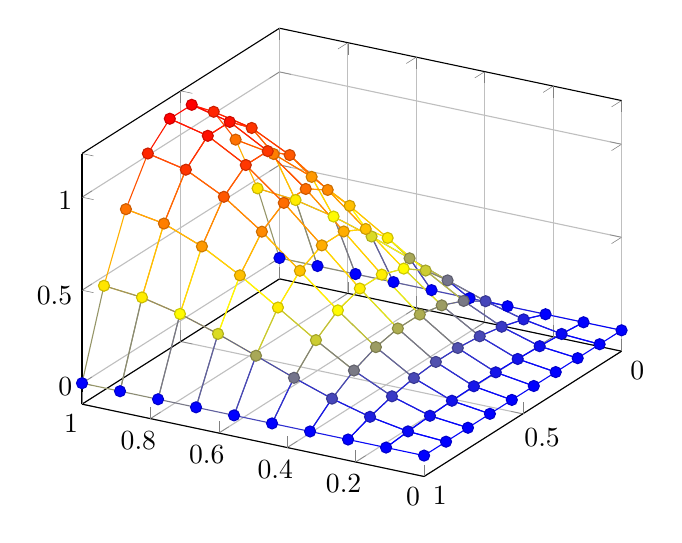
\begin{tikzpicture}
        \begin{axis}[grid=major,view={210}{30}]
        \addplot3+[mesh,scatter,samples=10,domain=0:1]
            {5*x*sin(2*deg(x)) * y*(1-y)};
        \end{axis}
    \end{tikzpicture}
}
%-------------------------------------------------------------------------------------------------------------------------------%
\def\@algorithmic@Test%
{%
    %\begin{algorithm}
%\caption{The Bellman-Kalaba algorithm}
\begin{algorithmic}[1]
\Procedure {BellmanKalaba}{$G$, $u$, $l$, $p$}
\ForAll {$v \in V(G)$}
\State $l(v) \leftarrow \infty$
\EndFor
\State $l(u) \leftarrow 0$
\Repeat \For {$i \leftarrow 1, n$}
\State $min \leftarrow l(v_i)$
\For {$j \leftarrow 1, n$}
\If {$min > e(v_i, v_j) + l(v_j)$}
\State $min \leftarrow e(v_i, v_j) + l(v_j)$
\State $p(i) \leftarrow v_j$
\EndIf
\EndFor
\State $l'(i) \leftarrow min$
\EndFor
\State $changed \leftarrow l \not= l'$
\State $l \leftarrow l'$
\Until{$\neg changed$}
\EndProcedure
\Statex
\Procedure {FindPathBK}{$v$, $u$, $p$}
\If {$v = u$}
\State \textbf{Write} $v$
\Else
\State $w \leftarrow v$
\While {$w \not= u$}
\State \textbf{Write} $w$
\State $w \leftarrow p(w)$
\EndWhile
\EndIf
\EndProcedure
\end{algorithmic}
%\end{algorithm}
}
%-------------------------------------------------------------------------------------------------------------------------------%
%~~~~~~~~~~~~~~~~~~~~~~~~~~~~~~~~~~~~~~~~~~~~~~~~~~~~~~~~~~~~~~~~~~~~~~~~~~~~~~~~~~~~~~~~~~~~~~~~~~~~~~~~~~~~~~~~~~~~~~~~~~~~~~~%
%~~~~~~~~~~~~~~~~~~~~~~~~~~~~~~~~~~~~~~~~~~~~~~~~~~~~~~~~~~~~~~~~~~~~~~~~~~~~~~~~~~~~~~~~~~~~~~~~~~~~~~~~~~~~~~~~~~~~~~~~~~~~~~~%
%~~~~~~~~~~~~~~~~~~~~~~~~~~~~~~~~~~~~~~~~~~~~~~~~~~~~~~~~~~~~~~~~~~~~~~~~~~~~~~~~~~~~~~~~~~~~~~~~~~~~~~~~~~~~~~~~~~~~~~~~~~~~~~~%
%-------------------------------------------------------------------------------------------------------------------------------%
\mathon
%-------------------------------------------------------------------------------------------------------------------------------%

%-------------------------------------------------------------------------------------------------------------------------------%
\mathoff
%-------------------------------------------------------------------------------------------------------------------------------%
%*******************************************************************************************************************************%
%************************************************** END of 'cs-examples.tex' ***************************************************%
%*******************************************************************************************************************************%
%-------------------------------------------------------------------------------------------------------------------------------%
% Restore @ -> \catcode'@=12 (active), peventing user access to macro names containing @ character
\makeatother
\endinput
%-------------------------------------------------------------------------------------------------------------------------------%
%*******************************************************************************************************************************%
%*********************************************************** NOTES *************************************************************%
%*******************************************************************************************************************************%
